%  LaTeX support: latex@mdpi.com
%  In case you need support, please attach all files that are necessary for compiling as well as the log file, and specify the details of your LaTeX setup (which operating system and LaTeX version / tools you are using).

%=================================================================
\documentclass[water,article,submit,moreauthors,pdftex]{mdpi}

% If you would like to post an early version of this manuscript as a preprint, you may use preprint as the journal and change 'submit' to 'accept'. The document class line would be, e.g., \documentclass[preprints,article,accept,moreauthors,pdftex]{mdpi}. This is especially recommended for submission to arXiv, where line numbers should be removed before posting. For preprints.org, the editorial staff will make this change immediately prior to posting.

%% Some pieces required from the pandoc template
\setlist[itemize]{leftmargin=*,labelsep=5.8mm}
\setlist[enumerate]{leftmargin=*,labelsep=4.9mm}


%--------------------
% Class Options:
%--------------------
%----------
% journal
%----------
% Choose between the following MDPI journals:
% acoustics, actuators, addictions, admsci, aerospace, agriculture, agriengineering, agronomy, algorithms, animals, antibiotics, antibodies, antioxidants, applsci, arts, asc, asi, atmosphere, atoms, axioms, batteries, bdcc, behavsci , beverages, bioengineering, biology, biomedicines, biomimetics, biomolecules, biosensors, brainsci , buildings, cancers, carbon , catalysts, cells, ceramics, challenges, chemengineering, chemistry, chemosensors, children, cleantechnol, climate, clockssleep, cmd, coatings, colloids, computation, computers, condensedmatter, cosmetics, cryptography, crystals, dairy, data, dentistry, designs , diagnostics, diseases, diversity, drones, econometrics, economies, education, electrochem, electronics, energies, entropy, environments, epigenomes, est, fermentation, fibers, fire, fishes, fluids, foods, forecasting, forests, fractalfract, futureinternet, futurephys, galaxies, games, gastrointestdisord, gels, genealogy, genes, geohazards, geosciences, geriatrics, hazardousmatters, healthcare, heritage, highthroughput, horticulturae, humanities, hydrology, ijerph, ijfs, ijgi, ijms, ijns, ijtpp, informatics, information, infrastructures, inorganics, insects, instruments, inventions, iot, j, jcdd, jcm, jcp, jcs, jdb, jfb, jfmk, jimaging, jintelligence, jlpea, jmmp, jmse, jnt, jof, joitmc, jpm, jrfm, jsan, land, languages, laws, life, literature, logistics, lubricants, machines, magnetochemistry, make, marinedrugs, materials, mathematics, mca, medicina, medicines, medsci, membranes, metabolites, metals, microarrays, micromachines, microorganisms, minerals, modelling, molbank, molecules, mps, mti, nanomaterials, ncrna, neuroglia, nitrogen, notspecified, nutrients, ohbm, particles, pathogens, pharmaceuticals, pharmaceutics, pharmacy, philosophies, photonics, physics, plants, plasma, polymers, polysaccharides, preprints , proceedings, processes, proteomes, psych, publications, quantumrep, quaternary, qubs, reactions, recycling, religions, remotesensing, reports, resources, risks, robotics, safety, sci, scipharm, sensors, separations, sexes, signals, sinusitis, smartcities, sna, societies, socsci, soilsystems, sports, standards, stats, surfaces, surgeries, sustainability, symmetry, systems, technologies, test, toxics, toxins, tropicalmed, universe, urbansci, vaccines, vehicles, vetsci, vibration, viruses, vision, water, wem, wevj

%---------
% article
%---------
% The default type of manuscript is "article", but can be replaced by:
% abstract, addendum, article, benchmark, book, bookreview, briefreport, casereport, changes, comment, commentary, communication, conceptpaper, conferenceproceedings, correction, conferencereport, expressionofconcern, extendedabstract, meetingreport, creative, datadescriptor, discussion, editorial, essay, erratum, hypothesis, interestingimages, letter, meetingreport, newbookreceived, obituary, opinion, projectreport, reply, retraction, review, perspective, protocol, shortnote, supfile, technicalnote, viewpoint
% supfile = supplementary materials

%----------
% submit
%----------
% The class option "submit" will be changed to "accept" by the Editorial Office when the paper is accepted. This will only make changes to the frontpage (e.g., the logo of the journal will get visible), the headings, and the copyright information. Also, line numbering will be removed. Journal info and pagination for accepted papers will also be assigned by the Editorial Office.

%------------------
% moreauthors
%------------------
% If there is only one author the class option oneauthor should be used. Otherwise use the class option moreauthors.

%---------
% pdftex
%---------
% The option pdftex is for use with pdfLaTeX. If eps figures are used, remove the option pdftex and use LaTeX and dvi2pdf.

%=================================================================
\firstpage{1}
\makeatletter
\setcounter{page}{\@firstpage}
\makeatother
\pubvolume{xx}
\issuenum{1}
\articlenumber{5}
\pubyear{2019}
\copyrightyear{2019}
%\externaleditor{Academic Editor: name}
\history{Received: date; Accepted: date; Published: date}
\updates{yes} % If there is an update available, un-comment this line

%% MDPI internal command: uncomment if new journal that already uses continuous page numbers
%\continuouspages{yes}

%------------------------------------------------------------------
% The following line should be uncommented if the LaTeX file is uploaded to arXiv.org
%\pdfoutput=1

%=================================================================
% Add packages and commands here. The following packages are loaded in our class file: fontenc, calc, indentfirst, fancyhdr, graphicx, lastpage, ifthen, lineno, float, amsmath, setspace, enumitem, mathpazo, booktabs, titlesec, etoolbox, amsthm, hyphenat, natbib, hyperref, footmisc, geometry, caption, url, mdframed, tabto, soul, multirow, microtype, tikz

%=================================================================
%% Please use the following mathematics environments: Theorem, Lemma, Corollary, Proposition, Characterization, Property, Problem, Example, ExamplesandDefinitions, Hypothesis, Remark, Definition
%% For proofs, please use the proof environment (the amsthm package is loaded by the MDPI class).

%=================================================================
% Full title of the paper (Capitalized)
\Title{Full title of the paper (Capitalized)}

% Authors, for the paper (add full first names)
\Author{$^{}$}

% Authors, for metadata in PDF
\AuthorNames{}

% Affiliations / Addresses (Add [1] after \address if there is only one affiliation.)
\address{%
$^{1}$ \quad Statistical and Data Sciences Smith College Northampton, MA 01063; \\
$^{2}$ \quad ; \href{mailto:aacharya@smith.edu}{\nolinkurl{aacharya@smith.edu}}\\
$^{3}$ \quad ; \href{mailto:dcaravela@smith.edu}{\nolinkurl{dcaravela@smith.edu}}\\
$^{4}$ \quad ; \href{mailto:ekim89@smith.edu}{\nolinkurl{ekim89@smith.edu}}\\
$^{5}$ \quad ; \href{mailto:ekornberg@smith.edu}{\nolinkurl{ekornberg@smith.edu}}\\
$^{6}$ \quad ; \href{mailto:enesmith@smith.edu}{\nolinkurl{enesmith@smith.edu}}\\
}
% Contact information of the corresponding author
\corres{Correspondence: \href{mailto:leutnant@fh-muenster.de}{\nolinkurl{leutnant@fh-muenster.de}};
Tel.: +XX-000-00-0000.}

% Current address and/or shared authorship
\firstnote{Current address: Updated affiliation}
\secondnote{These authors contributed equally to this work.}






% The commands \thirdnote{} till \eighthnote{} are available for further notes

% Simple summary

% Abstract (Do not insert blank lines, i.e. \\)
\abstract{A variety of disciplines use risk assessment instruments to help humans
make data-driven decisions. Northpointe, a software company, created a
risk assessment instrument known as the Correctional Offender Management
Profiling for Alternative Sanctions (COMPAS). COMPAS uses various
behavioral and psychological metrics related to recidivism to assist
justice systems in assessing a defendant's potential recidivism risk.
ProPublica published an article which concludes that the biases in the
criminal justice system are reflected in the COMPAS software. Using a
human rights framework adopted from the organization Women at the Table,
we use various debiasing algorithms to analyze both sides of the
argument between Northpointe and ProPublica and determine the level and
extent of racial bias in the COMPAS algorithm.}

% Keywords

% The fields PACS, MSC, and JEL may be left empty or commented out if not applicable
%\PACS{J0101}
%\MSC{}
%\JEL{}

%%%%%%%%%%%%%%%%%%%%%%%%%%%%%%%%%%%%%%%%%%
% Only for the journal Diversity
%\LSID{\url{http://}}

%%%%%%%%%%%%%%%%%%%%%%%%%%%%%%%%%%%%%%%%%%
% Only for the journal Applied Sciences:
%\featuredapplication{Authors are encouraged to provide a concise description of the specific application or a potential application of the work. This section is not mandatory.}
%%%%%%%%%%%%%%%%%%%%%%%%%%%%%%%%%%%%%%%%%%

%%%%%%%%%%%%%%%%%%%%%%%%%%%%%%%%%%%%%%%%%%
% Only for the journal Data:
%\dataset{DOI number or link to the deposited data set in cases where the data set is published or set to be published separately. If the data set is submitted and will be published as a supplement to this paper in the journal Data, this field will be filled by the editors of the journal. In this case, please make sure to submit the data set as a supplement when entering your manuscript into our manuscript editorial system.}

%\datasetlicense{license under which the data set is made available (CC0, CC-BY, CC-BY-SA, CC-BY-NC, etc.)}

%%%%%%%%%%%%%%%%%%%%%%%%%%%%%%%%%%%%%%%%%%
% Only for the journal Toxins
%\keycontribution{The breakthroughs or highlights of the manuscript. Authors can write one or two sentences to describe the most important part of the paper.}

%\setcounter{secnumdepth}{4}
%%%%%%%%%%%%%%%%%%%%%%%%%%%%%%%%%%%%%%%%%%

% Pandoc syntax highlighting
\usepackage{color}
\usepackage{fancyvrb}
\newcommand{\VerbBar}{|}
\newcommand{\VERB}{\Verb[commandchars=\\\{\}]}
\DefineVerbatimEnvironment{Highlighting}{Verbatim}{commandchars=\\\{\}}
% Add ',fontsize=\small' for more characters per line
\usepackage{framed}
\definecolor{shadecolor}{RGB}{248,248,248}
\newenvironment{Shaded}{\begin{snugshade}}{\end{snugshade}}
\newcommand{\AlertTok}[1]{\textcolor[rgb]{0.94,0.16,0.16}{#1}}
\newcommand{\AnnotationTok}[1]{\textcolor[rgb]{0.56,0.35,0.01}{\textbf{\textit{#1}}}}
\newcommand{\AttributeTok}[1]{\textcolor[rgb]{0.77,0.63,0.00}{#1}}
\newcommand{\BaseNTok}[1]{\textcolor[rgb]{0.00,0.00,0.81}{#1}}
\newcommand{\BuiltInTok}[1]{#1}
\newcommand{\CharTok}[1]{\textcolor[rgb]{0.31,0.60,0.02}{#1}}
\newcommand{\CommentTok}[1]{\textcolor[rgb]{0.56,0.35,0.01}{\textit{#1}}}
\newcommand{\CommentVarTok}[1]{\textcolor[rgb]{0.56,0.35,0.01}{\textbf{\textit{#1}}}}
\newcommand{\ConstantTok}[1]{\textcolor[rgb]{0.00,0.00,0.00}{#1}}
\newcommand{\ControlFlowTok}[1]{\textcolor[rgb]{0.13,0.29,0.53}{\textbf{#1}}}
\newcommand{\DataTypeTok}[1]{\textcolor[rgb]{0.13,0.29,0.53}{#1}}
\newcommand{\DecValTok}[1]{\textcolor[rgb]{0.00,0.00,0.81}{#1}}
\newcommand{\DocumentationTok}[1]{\textcolor[rgb]{0.56,0.35,0.01}{\textbf{\textit{#1}}}}
\newcommand{\ErrorTok}[1]{\textcolor[rgb]{0.64,0.00,0.00}{\textbf{#1}}}
\newcommand{\ExtensionTok}[1]{#1}
\newcommand{\FloatTok}[1]{\textcolor[rgb]{0.00,0.00,0.81}{#1}}
\newcommand{\FunctionTok}[1]{\textcolor[rgb]{0.00,0.00,0.00}{#1}}
\newcommand{\ImportTok}[1]{#1}
\newcommand{\InformationTok}[1]{\textcolor[rgb]{0.56,0.35,0.01}{\textbf{\textit{#1}}}}
\newcommand{\KeywordTok}[1]{\textcolor[rgb]{0.13,0.29,0.53}{\textbf{#1}}}
\newcommand{\NormalTok}[1]{#1}
\newcommand{\OperatorTok}[1]{\textcolor[rgb]{0.81,0.36,0.00}{\textbf{#1}}}
\newcommand{\OtherTok}[1]{\textcolor[rgb]{0.56,0.35,0.01}{#1}}
\newcommand{\PreprocessorTok}[1]{\textcolor[rgb]{0.56,0.35,0.01}{\textit{#1}}}
\newcommand{\RegionMarkerTok}[1]{#1}
\newcommand{\SpecialCharTok}[1]{\textcolor[rgb]{0.00,0.00,0.00}{#1}}
\newcommand{\SpecialStringTok}[1]{\textcolor[rgb]{0.31,0.60,0.02}{#1}}
\newcommand{\StringTok}[1]{\textcolor[rgb]{0.31,0.60,0.02}{#1}}
\newcommand{\VariableTok}[1]{\textcolor[rgb]{0.00,0.00,0.00}{#1}}
\newcommand{\VerbatimStringTok}[1]{\textcolor[rgb]{0.31,0.60,0.02}{#1}}
\newcommand{\WarningTok}[1]{\textcolor[rgb]{0.56,0.35,0.01}{\textbf{\textit{#1}}}}

% tightlist command for lists without linebreak
\providecommand{\tightlist}{%
  \setlength{\itemsep}{0pt}\setlength{\parskip}{0pt}}

% From pandoc table feature
\usepackage{longtable,booktabs,array}
\usepackage{calc} % for calculating minipage widths
% Correct order of tables after \paragraph or \subparagraph
\usepackage{etoolbox}
\makeatletter
\patchcmd\longtable{\par}{\if@noskipsec\mbox{}\fi\par}{}{}
\makeatother
% Allow footnotes in longtable head/foot
\IfFileExists{footnotehyper.sty}{\usepackage{footnotehyper}}{\usepackage{footnote}}
\makesavenoteenv{longtable}



\begin{document}


%%%%%%%%%%%%%%%%%%%%%%%%%%%%%%%%%%%%%%%%%%

\hypertarget{version}{%
\section{Version}\label{version}}

This Rmd-skeleton uses the mdpi Latex template published 2019/02.
However, the official template gets more frequently updated than the
`rticles' package. Therefore, please make sure prior to paper
submission, that you're using the most recent .cls, .tex and .bst files
(available \href{http://www.mdpi.com/authors/latex}{here}).

\hypertarget{introduction}{%
\section{Introduction}\label{introduction}}

Women @ the Table, the sponsor organization for this project, is ``a
growing, global gender equality \& democracy CSO based in Geneva,
Switzerland focused on advancing feminist systems change by using the
prism of technology, innovation \& AI exercising leverage points in
technology, the economy, sustainability \& democratic governance''
\citep{noauthor_womenthetable_nodate}. We have been asked to collaborate
on their AI \& Equality \citep{noauthor_ai_nodate} initiative, tasked
with debiasing the COMPAS algorithm
\citep{noauthor_aif360datasetscompasdataset_2018} and producing a
corresponding data story that will be added to their library.

The Correctional Offender Management Profiling for Alternative Sanctions
(COMPAS) algorithm was created by the private for-profit company
Northpointe, also known by its parent company Equivant
\citep{equivant_faq_nodate}, to predict defendants' risk of recidivism.
It generates a score that classifies defendants' risk of recidivism as
either low, medium, or high \citep{angwin2016machine}. Jurisdictions
across the United States use the COMPAS risk assessment instrument. In
2016, ProPublica published a piece that analyzed the methods and
algorithms used by Northpointe to uncover racial biases in defendants'
scores \citep{angwin2016machine}. Their analysis looks at the
distribution of decile COMPAS scores among Black and white defendants.
ProPublica concludes, after using a statistical parity metric on false
positives or false negatives, that the algorithm is racially biased
\citep{larson2016we}. Northpointe denies the allegations of racial bias,
conducting their own analyses based on different statistical parity
metrics \citep{equivant_response_2018}. Since then, the two parties have
had several exchanges, maintaining their original arguments. Currently,
the two parties' disagreement focuses on pretrial Risk Assessment
Instruments (RAIs). ProPublica maintains that there are biases in the
outcome values, protected attributes, and covariates during
Northpointe's data processing phase. ProPublica accounts for these
biases in their analyses, and Northepointe's response, highlights how
ProPublica did not account for base rates of recidivism in their
analysis, which are important to understand initial percentages without
the presence of other information.

Our project builds on Women at the Table's various debiasing algorithms
to conduct our own analyses on the COMPAS dataset. Based on this
analysis, we employ a human rights framework to contribute to the
ongoing ProPublica and Northpointe debate and investigate whether or to
what extent there is racial bias in the COMPAS algorithm. With a solid
understanding of the two sides, we aim to pinpoint the shortcomings of
both arguments and correct them in our analyses. We will use various
machine learning algorithms including logistic regression, cross
validation, and lasso and ridge techniques to choose models. We will
summarize our results using the JupyterNotebook framework from Women at
the Table, to be used by members of the organization to teach in a
workshop setting. We hope that our findings will highlight the
importance of checking statistical analyses using varied methods and
contribute to the ongoing discussion of the effects of machine biases in
the justice system.

\hypertarget{data}{%
\section{Data}\label{data}}

The data we are using for this project is the COMPAS General Recidivism
Risk Scores dataset from ProPublica used in their original analysis
\citep{larson_propublicacompas-analysiscompas-scores-two-yearscsv_2022}.
The COMPAS dataset we are using is from AI Fairness 360 (AIF360) toolkit
\citep{noauthor_trusted-ai_360} which does the same initial
preprocessing as ProPublica. The raw data has 6,167 rows and each row
represents an arrest charge for a defendant. ProPublica's COMPAS data
includes the defendant's age, race, sex, what they were charged with,
and whether or not the defendant ultimately recidivated within a
two-year period after their arrest. For the purposes of our project,
which endeavors to evaluate the differing effects of the COMPAS
algorithm on white defendants and Black defendants, we have filtered the
data to only include individuals whose race is listed as Caucasian or
African-American. Our data therefore has 5,723 rows (Figure
\ref{fig:table snip}), with the below distributions of race (Figure
\ref{fig:race plot}), age (Figure \ref{fig:age plot}), and two year
recidivism rate (Figures \ref{fig:recid plot} \&
\ref{fig:recid race plot}).

\begin{figure}

{\centering 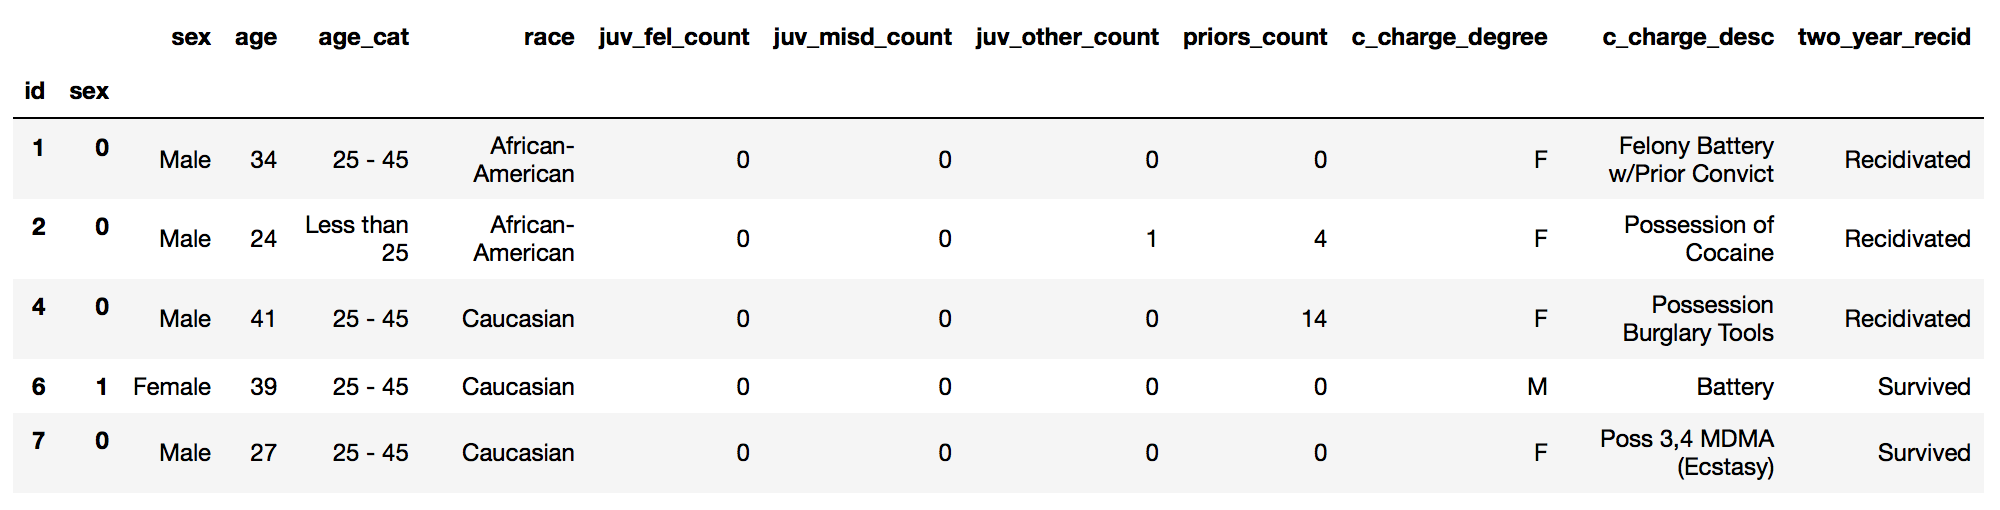
\includegraphics[width=400px,height=200px]{../images/table_snippet} 

}

\caption{This table is a snippet the data set we will be using.}\label{fig:table snip}
\end{figure}

\begin{figure}

{\centering 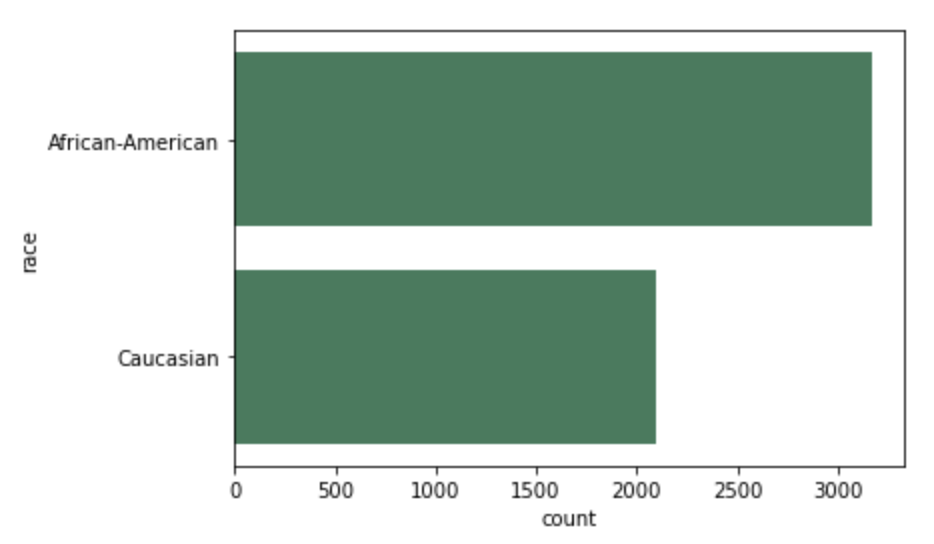
\includegraphics[width=400px,height=200px]{../images/race_bar_plot} 

}

\caption{This plot shows the distribution of defendant races.}\label{fig:race plot}
\end{figure}

\begin{figure}

{\centering 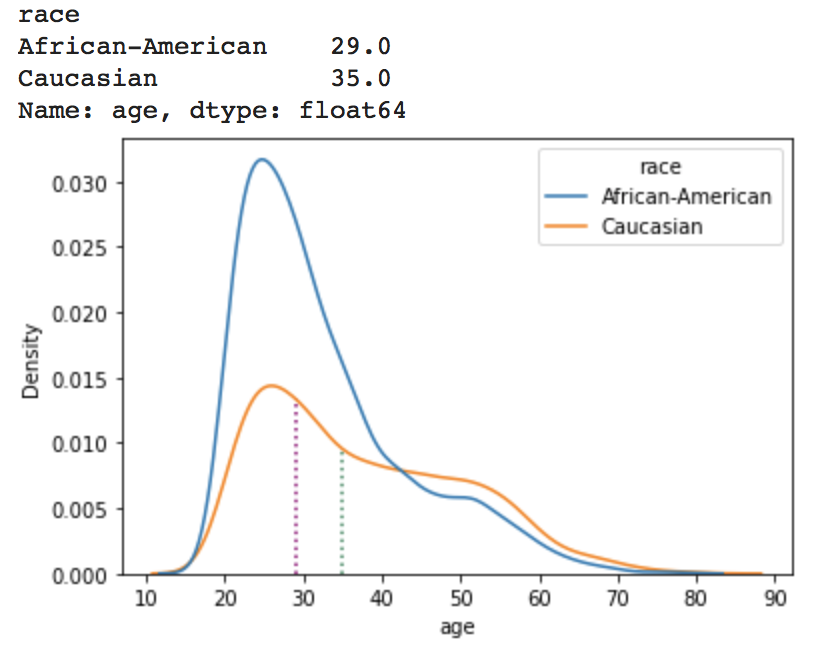
\includegraphics[width=400px,height=200px]{../images/race_age_plot} 

}

\caption{This plot shows the distribution of defendant ages by race.}\label{fig:age plot}
\end{figure}

\begin{figure}

{\centering 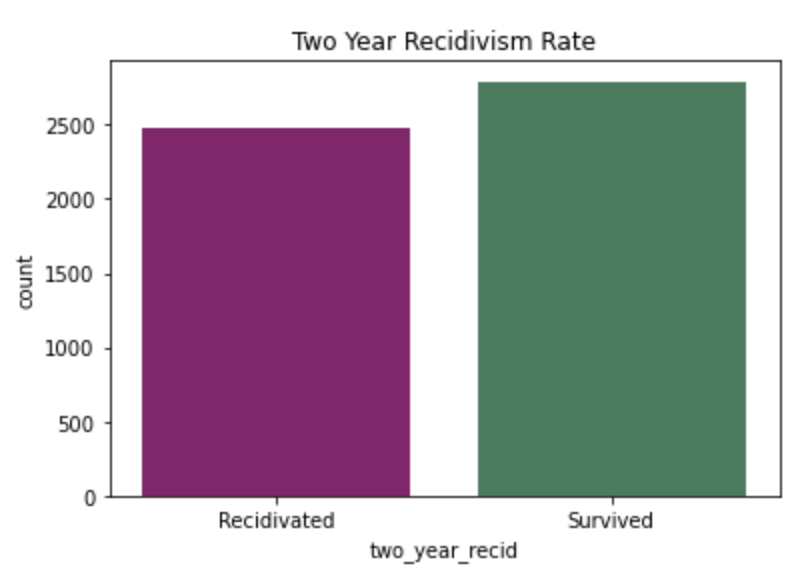
\includegraphics[width=400px,height=200px]{../images/recid_bar_plot} 

}

\caption{This plot shows the distribution of two year recidivism outcomes.}\label{fig:recid plot}
\end{figure}

\begin{figure}

{\centering 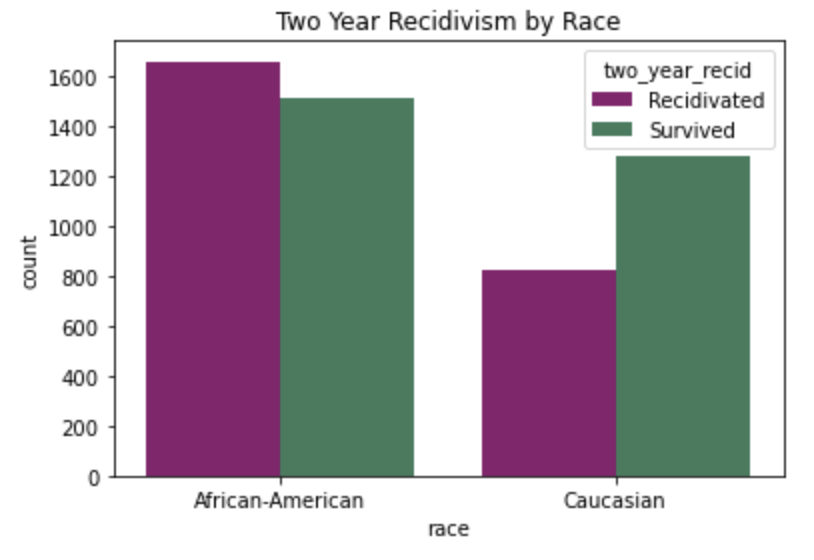
\includegraphics[width=400px,height=200px]{../images/race_recid_plot} 

}

\caption{This plot shows the distribution of two year recidivism outcomes by race.}\label{fig:recid race plot}
\end{figure}

\hypertarget{results}{%
\section{Results}\label{results}}

This section may be divided by subheadings. It should provide a concise
and precise description of the experimental results, their
interpretation as well as the experimental conclusions that can be
drawn.

\hypertarget{subsection-heading-here}{%
\subsection{Subsection Heading Here}\label{subsection-heading-here}}

Subsection text here.

\hypertarget{subsubsection-heading-here}{%
\subsubsection{Subsubsection Heading
Here}\label{subsubsection-heading-here}}

Bulleted lists look like this:

\begin{itemize}
\tightlist
\item
  First bullet
\item
  Second bullet
\item
  Third bullet
\end{itemize}

Numbered lists can be added as follows:

\begin{enumerate}
\def\labelenumi{\arabic{enumi}.}
\tightlist
\item
  First item
\item
  Second item
\item
  Third item
\end{enumerate}

The text continues here.

All figures and tables should be cited in the main text as Figure
\ref{fig:mdpi-logo}, Table 1, etc.

\begin{figure}

{\centering 
\includegraphics{logo-mdpi} 

}

\caption{This is a figure, Schemes follow the same formatting. If there are multiple panels, they should be listed as: (\textbf{a}) Description of what is contained in the first panel. (\textbf{b}) Description of what is contained in the second panel. Figures should be placed in the main text near to the first time they are cited. A caption on a single line should be centered.}\label{fig:mdpi-logo}
\end{figure}

Please see Table \ref{tab:mytable}.

\begin{Shaded}
\begin{Highlighting}[]
\NormalTok{x <-}\StringTok{ }\NormalTok{tibble}\OperatorTok{::}\KeywordTok{tribble}\NormalTok{(}\OperatorTok{~}\StringTok{`}\DataTypeTok{Title 1}\StringTok{`}\NormalTok{, }\OperatorTok{~}\StringTok{`}\DataTypeTok{Title 2}\StringTok{`}\NormalTok{, }\OperatorTok{~}\StringTok{`}\DataTypeTok{Title 3}\StringTok{`}\NormalTok{,}
\StringTok{"entry 1"}\NormalTok{, }\StringTok{"data"}\NormalTok{, }\StringTok{"data"}\NormalTok{,}
\StringTok{"entry 2"}\NormalTok{, }\StringTok{"data"}\NormalTok{, }\StringTok{"data"}
\NormalTok{)}

\NormalTok{knitr}\OperatorTok{::}\KeywordTok{kable}\NormalTok{(x, }\DataTypeTok{caption =} \StringTok{"This is a table caption. Tables should be placed in the main text near to the first time they are cited.}\CharTok{\textbackslash{}\textbackslash{}}\StringTok{label\{tab:mytable\}"}\NormalTok{)}
\end{Highlighting}
\end{Shaded}

\begin{longtable}[]{@{}lll@{}}
\caption{This is a table caption. Tables should be placed in the main
text near to the first time they are
cited.\label{tab:mytable}}\tabularnewline
\toprule
Title 1 & Title 2 & Title 3\tabularnewline
\midrule
\endfirsthead
\toprule
Title 1 & Title 2 & Title 3\tabularnewline
\midrule
\endhead
entry 1 & data & data\tabularnewline
entry 2 & data & data\tabularnewline
\bottomrule
\end{longtable}

This is an example of an equation:

\begin{equation}
\mathbb{S}
\end{equation}

Example of a theorem:

\begin{Theorem}
Example text of a theorem.
\end{Theorem}

The text continues here. Proofs must be formatted as follows:

Example of a proof:

\begin{proof}[Proof of Theorem 1]
Text of the proof. Note that the phrase `of Theorem 1' is optional if it is clear which theorem is being referred to.
\end{proof}

The text continues here.

\hypertarget{discussion}{%
\section{Discussion}\label{discussion}}

Authors should discuss the results and how they can be interpreted in
perspective of previous studies and of the working hypotheses. The
findings and their implications should be discussed in the broadest
context possible. Future research directions may also be highlighted.

\hypertarget{conclusion}{%
\section{Conclusion}\label{conclusion}}

This section is not mandatory, but can be added to the manuscript if the
discussion is unusually long or complex.

\hypertarget{bibliography}{%
\section{Bibliography}\label{bibliography}}

\citet{angwin2016machine} \citet{bao2021s} \citet{barocas2017fairness}
\citet{baumer2017texts} \citet{equivant_response_2018}
\citet{gebru2021datasheets} \citet{hardin2015data}
\citet{james2013introduction} \citet{knight2020automated}
\citet{kypraiou_what_2021} \citet{larson2016technical}
\citet{larson2016we} \citet{noauthor_ai_nodate}
\citet{noauthor_aif360datasetscompasdataset_2018}
\citet{noauthor_trusted-ai_360}
\citet{noauthor_propublicacompas-analysis_2022}
\citet{noauthor_womenthetable_nodate} \citet{vartan_1st_2022}

% %%%%%%%%%%%%%%%%%%%%%%%%%%%%%%%%%%%%%%%%%%
% %% optional
% \supplementary{The following are available online at www.mdpi.com/link, Figure S1: title, Table S1: title, Video S1: title.}
%
% % Only for the journal Methods and Protocols:
% % If you wish to submit a video article, please do so with any other supplementary material.
% % \supplementary{The following are available at www.mdpi.com/link: Figure S1: title, Table S1: title, Video S1: title. A supporting video article is available at doi: link.}

\vspace{6pt}

%%%%%%%%%%%%%%%%%%%%%%%%%%%%%%%%%%%%%%%%%%

%%%%%%%%%%%%%%%%%%%%%%%%%%%%%%%%%%%%%%%%%%

%%%%%%%%%%%%%%%%%%%%%%%%%%%%%%%%%%%%%%%%%%

%%%%%%%%%%%%%%%%%%%%%%%%%%%%%%%%%%%%%%%%%%
%% optional

\input{"appendix.tex"}

%%%%%%%%%%%%%%%%%%%%%%%%%%%%%%%%%%%%%%%%%%
% Citations and References in Supplementary files are permitted provided that they also appear in the reference list here.

%=====================================
% References, variant A: internal bibliography
%=====================================
%\reftitle{References}
%\begin{thebibliography}{999}
% Reference 1
%\bibitem[Author1(year)]{ref-journal}
%Author1, T. The title of the cited article. {\em Journal Abbreviation} {\bf 2008}, {\em 10}, 142--149.
% Reference 2
%\bibitem[Author2(year)]{ref-book}
%Author2, L. The title of the cited contribution. In {\em The Book Title}; Editor1, F., Editor2, A., Eds.; Publishing House: City, Country, 2007; pp. 32--58.
%\end{thebibliography}

% The following MDPI journals use author-date citation: Arts, Econometrics, Economies, Genealogy, Humanities, IJFS, JRFM, Laws, Religions, Risks, Social Sciences. For those journals, please follow the formatting guidelines on http://www.mdpi.com/authors/references
% To cite two works by the same author: \citeauthor{ref-journal-1a} (\citeyear{ref-journal-1a}, \citeyear{ref-journal-1b}). This produces: Whittaker (1967, 1975)
% To cite two works by the same author with specific pages: \citeauthor{ref-journal-3a} (\citeyear{ref-journal-3a}, p. 328; \citeyear{ref-journal-3b}, p.475). This produces: Wong (1999, p. 328; 2000, p. 475)

%=====================================
% References, variant B: external bibliography
%=====================================
\reftitle{References}
\externalbibliography{yes}
\bibliography{mybibfile.bib}

%%%%%%%%%%%%%%%%%%%%%%%%%%%%%%%%%%%%%%%%%%
%% optional

%% for journal Sci
%\reviewreports{\\
%Reviewer 1 comments and authors’ response\\
%Reviewer 2 comments and authors’ response\\
%Reviewer 3 comments and authors’ response
%}

%%%%%%%%%%%%%%%%%%%%%%%%%%%%%%%%%%%%%%%%%%


\end{document}

